\documentclass{article}
\usepackage[table]{xcolor}
\usepackage{titlepic}
\usepackage{hyperref}
\usepackage{amsmath}
\usepackage{enumitem}% http://ctan.org/pkg/enumerate
\usepackage{rotating} 
\usepackage{float}
\usepackage{multirow}
\usepackage[margin=0.5in]{geometry}
\usepackage{titling}
\usepackage{capt-of}
\usepackage{siunitx}
%\usepackage{arydshln}
\usepackage{longtable}
\usepackage{xcolor}
\usepackage{colortbl}
%\usepackage[justification=centering]{caption}
%\usepackage{caption}
\sisetup{group-separator = {,}, group-minimum-digits = 4}
\definecolor{CSONavy}{HTML}{405381}
\hypersetup{
    colorlinks,
    linkcolor={black!50!black},
    citecolor={blue!50!black},
    urlcolor={blue!80!black}
}
\urlstyle{same}
%\nocite{*}
%\setlength{\droptitle}{-4.5em}

%\titlepic{
\includegraphics{../figures/CSO_Logo.png}}
\title{CHN Health Profile - West Mayo (IHA: HSE Mayo ;  Health Region: HSE West and North West) }
%\date{\vspHRe{-5ex}}
\date{Census 2022}
\author{CSO, Ireland  (\url{http://www.cso.ie)}}

\newcolumntype{T}{>{\raggedleft\arraybackslash}m{1.7cm}}
\newcolumntype{O}{>{\centering\arraybackslash}m{3.4cm}}
\newcolumntype{M}{>{\raggedleft\arraybackslash}m{3cm}}
\newcolumntype{A}{>{\raggedright\arraybackslash}m{9.5cm}}
\newcolumntype{S}{>{\raggedleft\arraybackslash}m{1.4cm}}
\newcolumntype{K}{>{\raggedright\arraybackslash}m{7.5cm}}

\usepackage{Sweave}
\begin{document}
\Sconcordance{concordance:54-west-mayo_hse-west-and-north-west.tex:HealthProfileTemplate.Rnw:1 44 1 1 0 %
889 1}

%
\includegraphics{../figures/CSO_Logo.png}
%\begin{minipage}{\linewidth}

\begin{figure}
	\centering

\includegraphics[width =75mm]{../figures/CSO_Logo.png}
\end{figure}

				 
		   
						  
														  
																																													
												 
			 
\maketitle
					
													   
				 
						 
																																																																											   
				 
				  
  \pagebreak
    	    \tableofcontents
%\end{minipage}

\pagebreak


\section{Key Points}


\begin{itemize}

\item The \textbf{Age Dependency Ratio} of this CHN is  \textbf{64.8}. This compares to 53.2 nationally. The Age Dependency Ratio is the amount of people outside of working age (0-14 and 65+) per 100 people of working age (15-64). 

\item West Mayo has a total of \textbf{\num{37368}} \textbf{persons} and  \textbf{\num{9436}} \textbf{families} living in private households.

\item There are a total of \textbf{\num{7107} persons aged 0-14} in this CHN and \textbf{\num{7583} persons aged over 65.} 

\item There are a total of \textbf{\num{8029}} persons \textbf{living with a disability} in this CHN, representing \textbf{21.5 percent} of the population. This compares with  21.5 percent nationally

\item \textbf{\num{650}} people in this CHN have \textbf{bad or very bad general health}. This represents \textbf{1.7 percent} of the population. 1.7 percent of the population have bad or very bad general health nationally. 

\item There are a total of \textbf{\num{2667} carers} in this CHN, representing \textbf{7.1 percent} of the population. This compares with 5.8 percent of the population that are carers nationally. 

\item \textbf{12.1 percent} of this CHN \textbf{smoke tobacco products}. 13.1 percent of people nationally smoke tobacco products

\item There are \textbf{\num{454} short term unemployed} and \textbf{\num{664} long term unemployed} people in this CHN. These represent 1.5 and 2.2 percent of the population respectively.

\item  \textbf{3.5 percent} of the population of West Mayo are \textbf{unskilled}. 3.1 percent of people in the state are unskilled.

\item \textbf{25.1 percent} of those aged 15+ in this CHN have a \textbf{highest level of education of lower secondary or lower}. This compares with 23 percent nationally. 

\item \textbf{22.1 percent} of families with children in this CHN have \textbf{lone parents}. This stands at 24.8 nationally.

\item \textbf{18.7 percent} of this CHN were \textbf{born outside Ireland} (20 percent nationally).

\item \textbf{Households rented from a Local Authority} comprise \textbf{4.4 percent} of households in this CHN.This stands at 8.3 percent nationally

\end{itemize}

\pagebreak

\section{Population} 
\label{sect:Pop}

\begin{figure}[h]
	\centering
	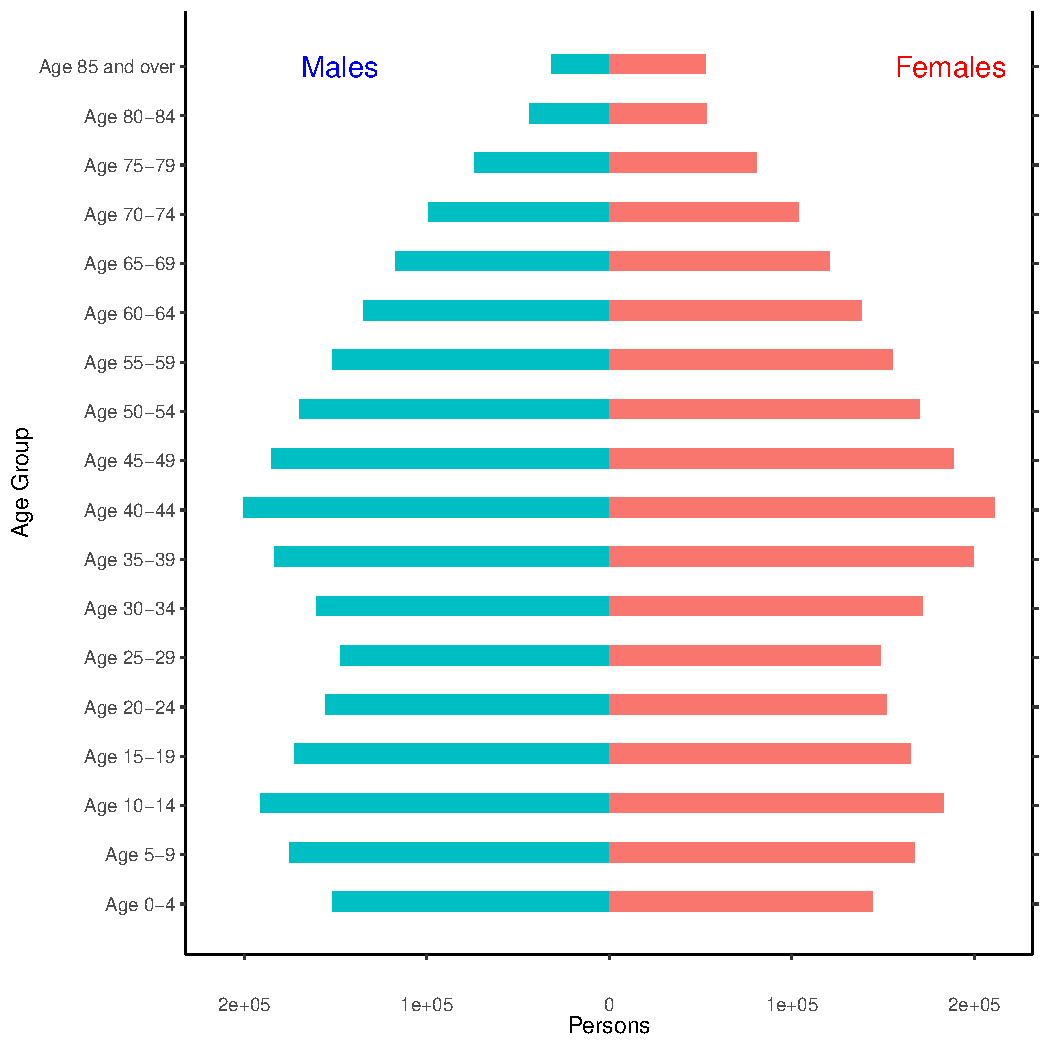
\includegraphics[width = 100mm]{../figures/PyramidPlot.pdf}
	\caption{Persons by Age Group and Gender for West Mayo; Census 2022.}
	\label{fig:2ae19629-1a6a-13a3-e055-000000000001}
	\end{figure}

\begin{table}[!h]
\centering
\begin{tabular}{lSSSSSSSSSS}
  \hline
 \textbf{Age} & \multicolumn{2}{c}{\textbf{Females}} & \multicolumn{2}{c}{\textbf{Males }} & \multicolumn{4}{c}{\textbf{Both Sexes}}  \\ 
\cline{6-9}\\
 & \emph{\textbf{Persons}} & \emph{\textbf{\%}} & \emph{\textbf{Persons}} & \emph{\textbf{\%}} & \emph{\textbf{Persons}} & \emph{\textbf{\% (CHN)}} & \emph{\textbf{\% (IHA)}}& \emph{\textbf{\% (State)}}\\
  \hline
  0-14   & 3477 &  18.4 & 3630 & 19.7 & 7107 &19.0 & 19.1& 19.7 \\
  15-64  & 11537 & 60.9 & 11141 & 60.5 & 22678&60.7& 61.1  &65.3\\
  65+ & 3926 & 20.7 & 3657 & 19.8 &7583 &20.3 & 19.8& 15.1 \\
 \hline
  Age 0-4  & 1038& 5.5& 1028 & 5.6& 2066 & 5.5 & 5.6&  5.7 \\
  
  Age 5-9  & 1153& 6.1& 1279 & 6.9& 2432 & 6.5 & 6.5&  6.7 \\

  Age 10-14  & 1286& 6.8& 1323 & 7.2& 2609 & 7.0 & 7.0&  7.3 \\

  Age 15-19  & 1132& 6.0& 1197 & 6.5& 2329 & 6.2 & 6.3& 6.6 \\

  Age 20-24  & 761& 4.0& 824 & 4.5& 1585 & 4.2 & 4.5&  6.0 \\

  Age 25-29  & 744& 3.9& 748 & 4.1& 1492 & 4.0& 4.2 & 5.7 \\

  Age 30-34  & 970& 5.1& 908 & 4.9& 1878 & 5.0 & 5.4&  6.5 \\

  Age 35-39  & 1269& 6.7& 1132 & 6.1& 2401 & 6.4 & 6.7&  7.4 \\

  Age 40-44  & 1511& 8.0& 1350 & 7.3& 2861 & 7.7 & 7.2&  8.0 \\
  
    Age 45-49  & 1336& 7.1& 1309 & 7.1& 2645 & 7.1 & 6.8&  7.3 \\
  
    Age 50-54  & 1320& 7.0& 1276 & 6.9& 2596 & 6.9 & 6.8&  6.6 \\
  
    Age 55-59  & 1279& 6.8& 1248 & 6.8& 2527 & 6.8 & 6.7&  6.0 \\
  
    Age 60-64  & 1215& 6.4& 1149 & 6.2& 2364 & 6.3 & 6.5&  5.3 \\
  
    Age 65-69  & 1163& 6.1& 1165 & 6.3& 2328 & 6.2 & 6.0&  4.6 \\
  
    Age 70-74  & 1010& 5.3& 1017 & 5.5& 2027 & 5.4 & 5.3&  3.9 \\
  
    Age 75-79  & 753& 4.0& 749 & 4.1& 1502 & 4.0 & 3.8&  3.0 \\
  
    Age 80-84  & 479& 2.5& 433 & 2.3& 912 & 2.4 & 2.4&  1.9\\
  
    Age 85 and over  & 521& 2.8& 293 & 1.6& 814 & 2.2 & 2.2 & 1.6 \\
  
    All Ages  & 18940& 100.0& 18428 & 100.0& 37368 & 100.0 & 100.0& 100.0 \\
      \hline 
    \multicolumn{4}{l}{\href{https://data.cso.ie/table/SAP2022T1T1AED}{https://data.cso.ie/table/SAP2022T1T1AED}} & &
\end{tabular}
\caption{Population Breakdown by Age and Sex for West Mayo; Census 2022. Percentage breakdowns for IHA, Health Region (HR) and State are provided for comparison purposes.}
\end{table}
\begin{itemize}
\item This CHN ranks  49  out of 96 regarding the percentage of persons aged 0 - 14, while it ranks  3 out of 3 CHNs in its IHA
\item This CHN ranks  49 out of 96 regarding the percentage of persons aged 65+, while it ranks   3 out of 3 CHNs in its IHA
\end{itemize}
\pagebreak


\section{Disability}\label{sect:Disability}

\begin{itemize}
\item This CHN ranks  29 out of 96 regarding the percentage of males with a disability, while it ranks  1 out of 3 CHNs in its IHA
\item This CHN ranks  28 out of 96 regarding the percentage of females with a disability, while it ranks   2 out of 3 CHNs in its IHA.
\end{itemize}

\begin{figure}[h]
	\centering
	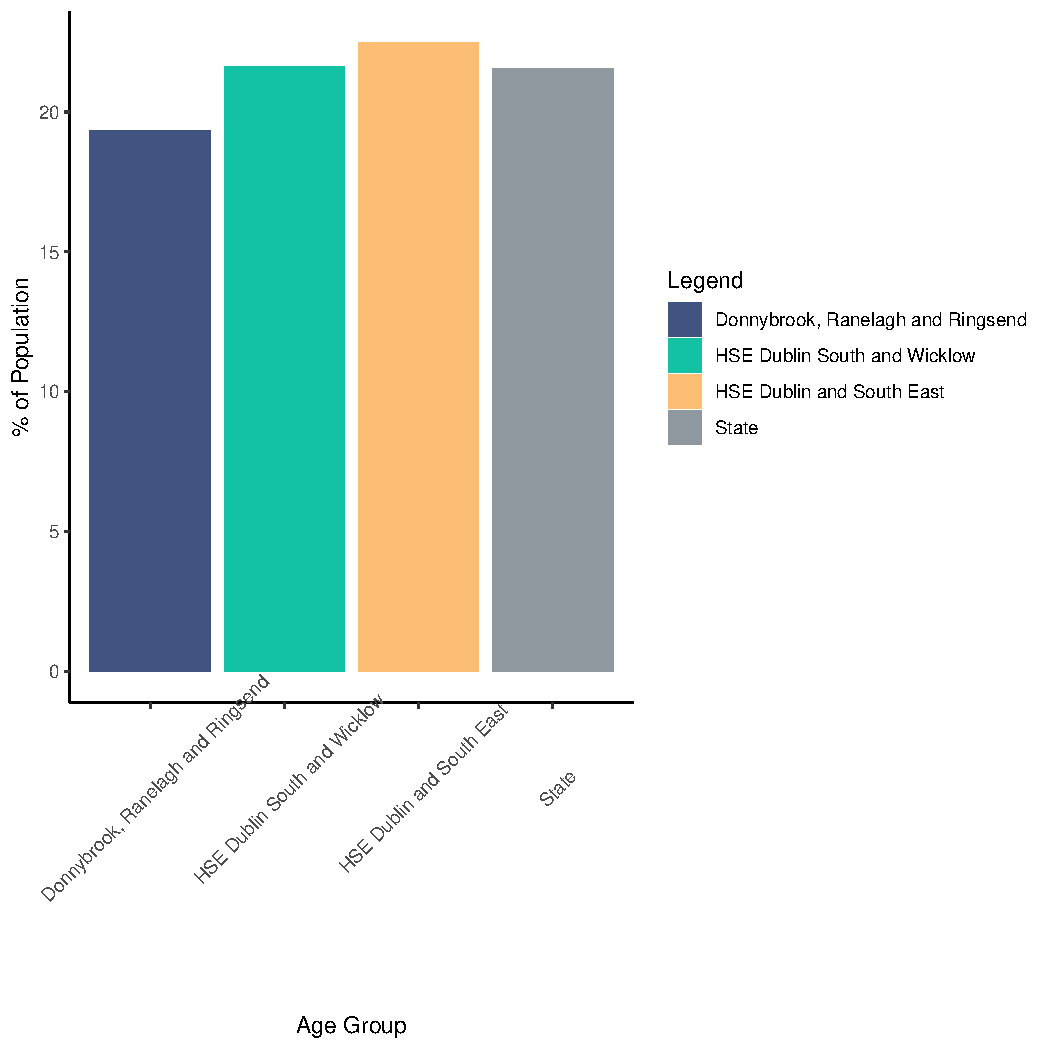
\includegraphics[width = 130mm]{../figures/DisED.pdf}
	\caption{Percentage of Population with any Disability by Age Group for West Mayo; IHA, Health Region and State; Census 2022.}
	\label{fig:2ae19629-1a6a-13a3-e055-000000000001}
	\end{figure}


\begin{table}[!h]
\centering
\begin{tabular}{lTTTTTT}
  \hline
 & \multicolumn{3}{c}{\textbf{West Mayo}} & \textbf{IHA}& \textbf{HR} & \textbf{State}\\ 
 \cline{2-4} \\
  \textbf{Age Group} & \textbf{Population} & \multicolumn{4}{c}{\textbf{With any Disability}} \\
 \cline{3-7}\\
& \emph{\textbf{Persons}} & \emph{\textbf{Persons}} & \emph{\textbf{\%}} & \emph{\textbf{\%}} & \emph{\textbf{\%}}& \emph{\textbf{\%}}\\
  \hline
Males & \num{18428} & \num{3851}  & 20.9  & 21.2 & 21.3 & 20.9\\
Females & \num{18940} & \num{4178}  & 22.1  & 22.4& 22.3& 22.2\\
Both Sexes & \num{37368} & \num{8029}  & 21.5  & 22.4& 22.3& 21.5 \\
   \hline
       \multicolumn{5}{l}{\href{https://data.cso.ie/table/F4004}{https://data.cso.ie/table/F4004}} & 
\end{tabular}
\caption{Population with any Disability by Age Group for West Mayo; Census 2022. Percentage breakdowns for IHA, Health Region and State are provided for comparison purposes.}
\end{table}

\pagebreak

\section{General Health}\label{sect:GenHealth}
\begin{itemize}
\item  This CHN ranks  16 out of 96 regarding the percentage of the population with bad or very bad General Health, while it ranks   3 out of 3 CHNs in its IHA.
\end{itemize}
\begin{figure}[h]
	\centering
	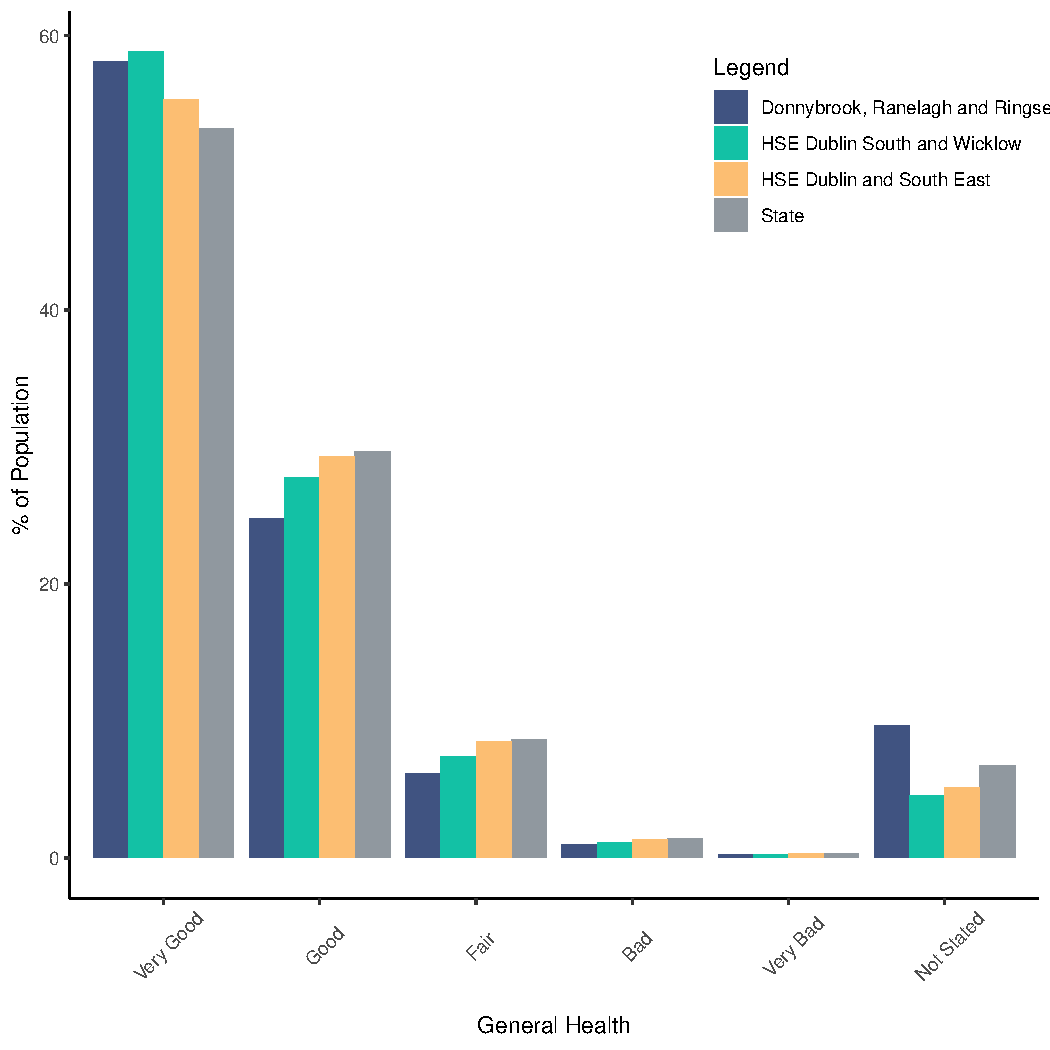
\includegraphics[width = 150mm]{../figures/GenED.pdf}
	\caption{Population Breakdown (\%) by General Health for West Mayo; IHA, Health Region and State;  Census 2022.}
	\label{fig:2ae19629-1a6a-13a3-e055-000000000001}
	\end{figure}

\begin{table}[!h]
\centering
\begin{tabular}{lTTTTT}
  \hline
\textbf{General Health} & \multicolumn{2}{c}{\textbf{West Mayo}} & \textbf{IHA}& \textbf{HR} & \textbf{State}\\ 
 \cline{2-3} \\
 & \emph{\textbf{Persons}} & \emph{\textbf{\%}} & \emph{\textbf{\%}} & \emph{\textbf{\%}}& \emph{\textbf{\%}} \\
  \hline
Very Good& \num{19492} &52.2
&51.4
&52.3 &53.2 \\
Good& \num{11951} &32.0 &32.1 &30.8 &29.7\\
Fair& \num{3545} &9.5 &10.2 &9.6 &8.6\\
Bad& \num{535} &1.4 &1.6 &1.5 &1.4\\
Very Bad& \num{115} &0.3 &0.3 &0.3 &0.3\\
Not Stated& \num{1730} &4.6 &4.5 &5.5 &6.7\\
Total& \num{37368} &100.0 &100.0 &100.0 &100.0\\
   \hline
       \multicolumn{5}{l}{\href{https://data.cso.ie/table/SAP2022T12T3ED}{https://data.cso.ie/table/SAP2022T12T3ED}} & 
\end{tabular}
\caption{Population by General Health for West Mayo; Census 2022. Percentage breakdowns for IHA, Health Region and State are also provided for comparison purposes.}
\end{table}
\pagebreak

\section{Carers}\label{sect:Carers}
\begin{itemize}
\item This CHN ranks  2 out of 96 regarding the percentage of males that are carers, while it ranks   1 out of 3 CHNs in its IHA.
\item This CHN ranks  5 out of 96 regarding the percentage of females that are carers, while it ranks   2 out of 3 CHNs in its IHA.
\end{itemize}
\begin{figure}[H]
	\centering
	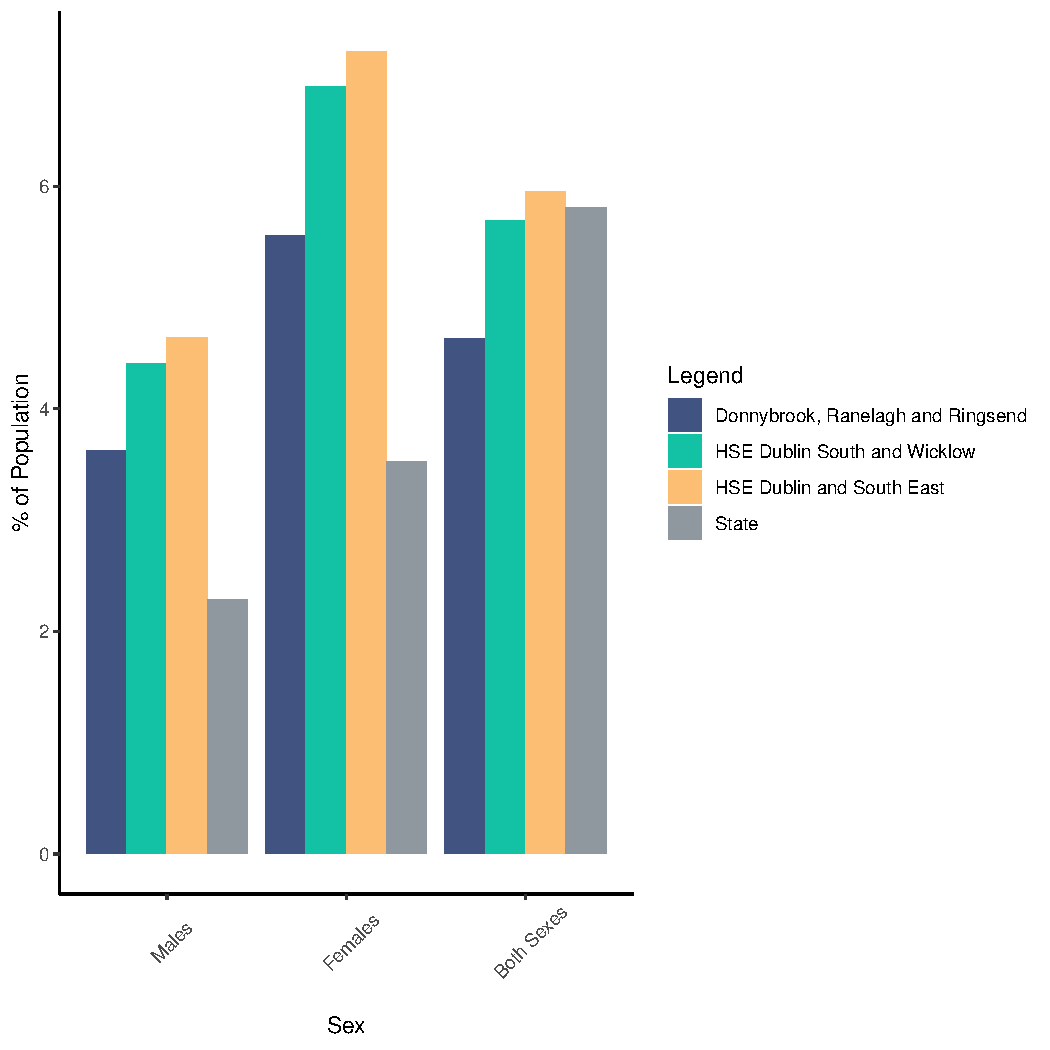
\includegraphics[width = 150mm]{../figures/CareED.pdf}
	\caption{Carers as a Percentage of the Population of Males/Females/Both Sexes for West Mayo; IHA, Health Region and State; Census 2022.}
	\label{fig:2ae19629-1a6a-13a3-e055-000000000001}
	\end{figure}
	\begin{table}[!h]	
\centering
	\begin{tabular}{lTTTTTT}
  \hline
 & \multicolumn{3}{c}{\textbf{West Mayo}} & \textbf{IHA}& \textbf{HR} & \textbf{State}\\ 
 \cline{2-4} \\
  \textbf{Age Group} & \textbf{Population} & \multicolumn{5}{c}{\textbf{Carers}} \\
 \cline{3-7}\\
& \emph{\textbf{Persons}} & \emph{\textbf{Persons}} & \emph{\textbf{\%}} & \emph{\textbf{\%}}& \emph{\textbf{\%}} & \emph{\textbf{\%}}\\
  \hline
Males & \num{18428} & \num{1107}  & 6.0  & 5.7  & 5.3 & 2.3 \\
Females & \num{18940} & \num{1560}  & 8.2  & 8.0 & 7.5 & 3.5 \\
Both Sexes & \num{37368} & \num{2667}  & 7.1  & 6.9& 6.4 & 5.8 \\
     \hline
       \multicolumn{3}{l}{\href{https://data.cso.ie/table/SAP2022T12T2ED}{https://data.cso.ie/table/SAP2022T12T2ED}} 
\end{tabular}

\caption{Carers by Sex for West Mayo; Census 2022. Percentage Breakdowns for IHA, Health Region and State are also provided for comparison purposes.}
\end{table} 



\pagebreak

\section{Volunteers}\label{sect:Volunteers}
\begin{itemize}
\item This CHN ranks  1 out of 96 regarding the percentage of the population that volunteer, while it ranks  1 out of 3 CHNs in its IHA.
\end{itemize}
\begin{figure}[H]
	\centering
	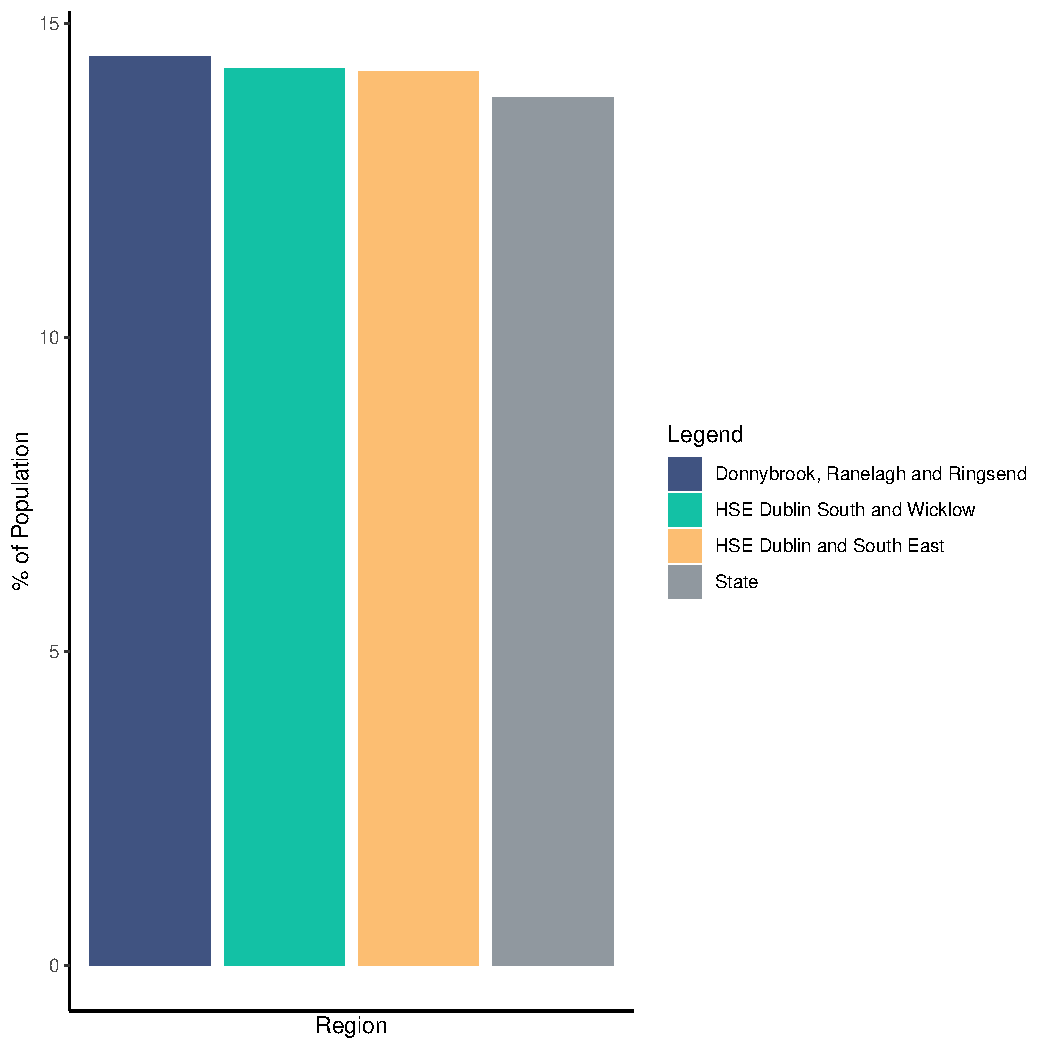
\includegraphics[width = 150mm]{../figures/VolunteerED.pdf}
	\caption{Volunteers as a Percentage of the Population for West Mayo; IHA, Health Region and State; Census 2022.}
	\label{fig:2ae19629-1a6a-13a3-e055-000000000001}
	\end{figure}
	
	
\begin{table}[!h]	
\centering
	\begin{tabular}{lTTTTTT}
  \hline
 & \multicolumn{3}{c}{\textbf{West Mayo}} & \textbf{IHA}& \textbf{HR} & \textbf{State}\\ 
 \cline{2-4} \\
  & \textbf{Population} & \multicolumn{5}{c}{\textbf{Volunteers}} \\
 \cline{3-7}\\
& \emph{\textbf{Persons}} & \emph{\textbf{Persons}} & \emph{\textbf{\%}} & \emph{\textbf{\%}}& \emph{\textbf{\%}} & \emph{\textbf{\%}}\\
  \hline 
& 37368 & 6909  & 18.5  & 16.9   & 15.6 & 13.8 \\

     \hline
       \multicolumn{3}{l}{\href{https://data.cso.ie/table/SAP2022T7T1ED}} 
\end{tabular}

\caption{Volunteers for West Mayo; Census 2022. Percentage Breakdowns for IHA, Health Region and State are also provided for comparison purposes.}
\end{table} 

\pagebreak

\section{Smoking}\label{sect:Smoking}
\begin{itemize}
\item This CHN ranks  34 out of 96 regarding the percentage of the population who smoke (daily and occasionally), while it ranks   2 out of 3 CHNs in its IHA.
\end{itemize}
\begin{figure}[H]
	\centering
	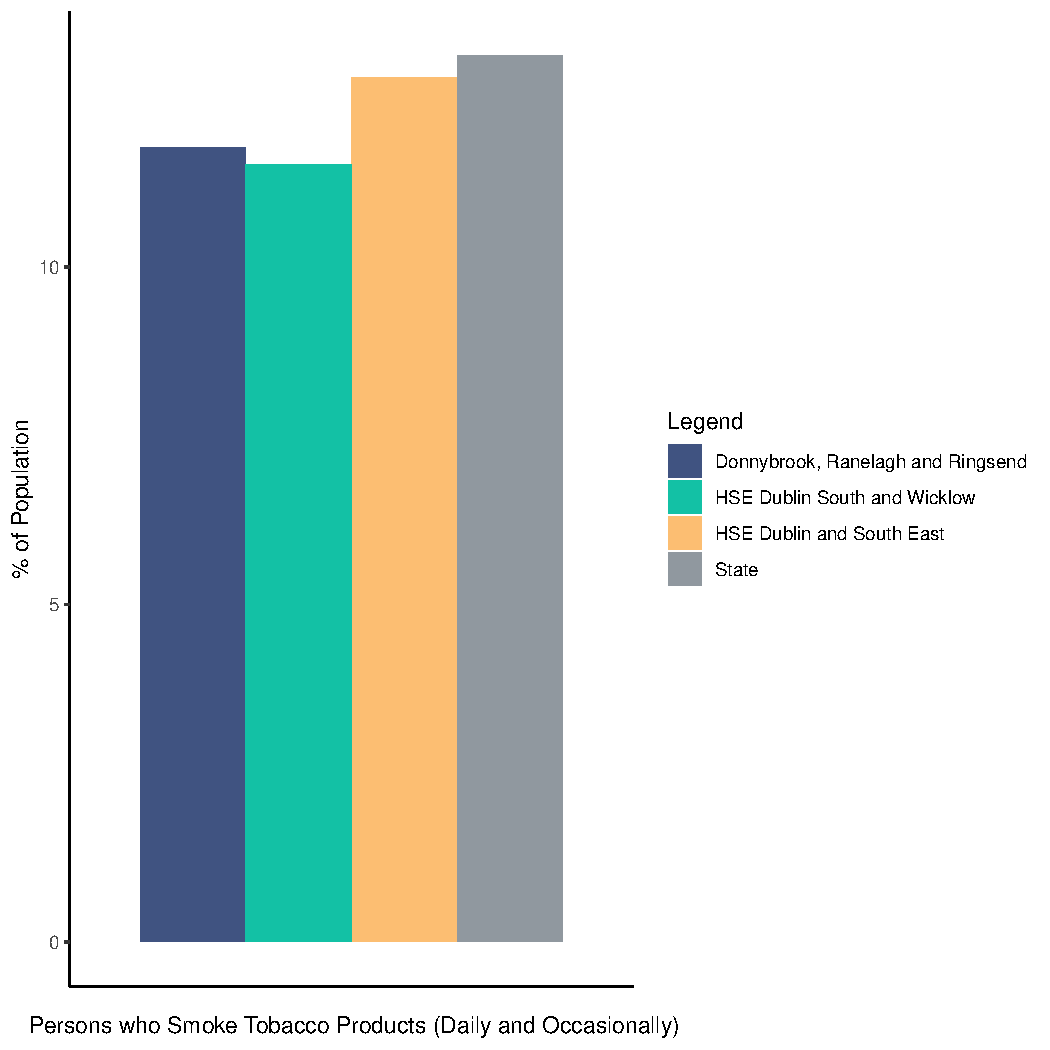
\includegraphics[width = 120mm]{../figures/SmokingED.pdf}
	\caption{Percentage of the Population who Smoke tobacco Products (Daily and Occasionally) for West Mayo; IHA, Health Region and State; Census 2022.}
	\label{fig:2ae19629-1a6a-13a3-e055-000000000001}
	\end{figure}
	
	
\begin{table}[!h]	
\centering
	\begin{tabular}{lTTTTTT}
  \hline
  \textbf{Smoking Status} & \multicolumn{2}{c}{\textbf{West Mayo}} & \textbf{IHA}& \textbf{HR} & \textbf{State}\\ 
 \cline{2-3} \\
 & \emph{\textbf{Persons}} & \emph{\textbf{\%}} & \emph{\textbf{\%}} & \emph{\textbf{\%}} & \emph{\textbf{\%}} \\
  \hline
Smoke tobacco Products (Daily and Occasionally)& \num{4540} &12.1 &12.4&12.5 &13.1 \\
Don't Smoke tobacco Products (Never and have given up)& \num{30807} &82.4 &82.4&81.2 &79.4 \\
Smoking Status Not Stated& \num{2021} &5.4 &5.3&6.3 &7.5 \\
All Persons & 37368 & 100.0 & 100.0  & 100.0  & 100.0\\
     \hline
      \multicolumn{3}{l}{\href{https://data.cso.ie/table/SAP2022T12T4ED}{https://data.cso.ie/table/SAP2022T12T4ED}} 
\end{tabular}

\caption{Smoking Status of West Mayo; Census 2022. Percentage breakdowns for IHA, Health Region and State are also provided for comparison purposes.}
\end{table} 
    
  
\pagebreak
\section{Principal Economic Status}\label{sect:PES}
\begin{figure}[H]
	\centering
	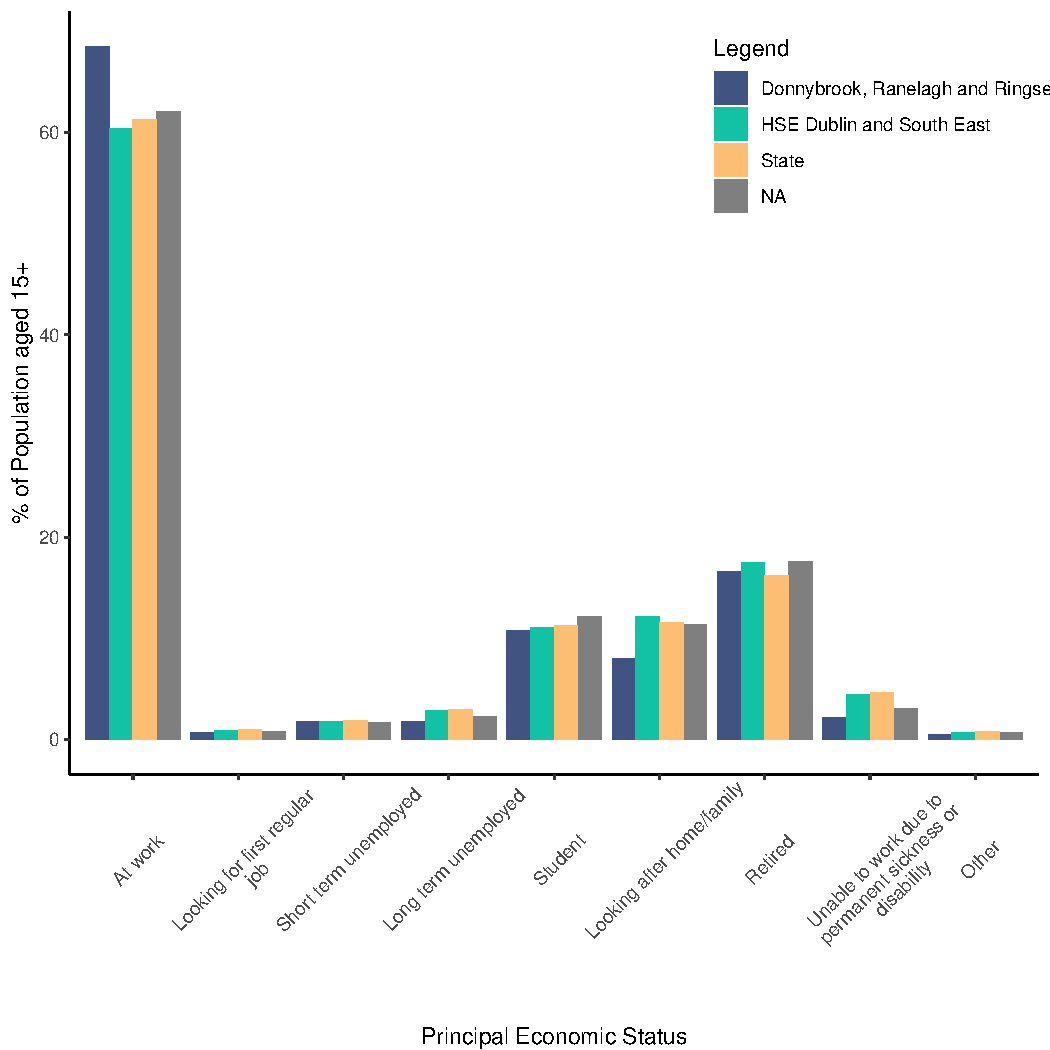
\includegraphics[width = 140mm]{../figures/PESED.pdf}
	\caption{Percentage of Population Aged 15+ by Principal Economic Status for West Mayo, IHA, Health Region and State; Census 2022.}
	\label{fig:vbnv}
	\end{figure}

\begin{table}[h]	
\centering
		\begin{tabular}{lTTTTTT}
  \hline
  \textbf{Principal Economic Status} & \multicolumn{2}{c}{\textbf{West Mayo}}& \textbf{IHA} & \textbf{HR} & \textbf{State}\\ 
 \cline{2-3} \\
 & \emph{\textbf{Persons}} & \emph{\textbf{\%}} & \emph{\textbf{\%}} & \emph{\textbf{\%}} & \emph{\textbf{\%}} \\
  \hline
At Work & \num{16238} &53.7
&52.3
&53.6 &56.1 \\
Looking for first regular job & \num{161} &0.5 &0.8&0.8 &0.8 \\
Short term unemployed & \num{454} &1.5 &1.6&1.7 &1.7 \\
Long term unemployed & \num{664} &2.2 &2.7&2.7 &2.6 \\
Student & \num{2893} &9.6
&9.7&11.1 &11.1 \\
 Looking after home/family & \num{1992} &6.6 &6.7&6.4 &6.6 \\
Retired & \num{6417} &21.2 &20.7 &18.4 &15.9 \\
Unable to work due to permanent sickness or disability & \num{1212} &4.0 &4.8&4.8 &4.6 \\
Other & \num{230} &0.8 &0.8 &0.7 &0.7 \\
Total & \num{30261} &100.0 &100.0 &100.0 &100.0 \\
\hline
       \multicolumn{5}{l}{\href{https://data.cso.ie/table/SAP2022T8T1ED}{https://data.cso.ie/table/SAP2022T8T1ED}} &
\end{tabular}
\caption{Population aged 15+ by Principal Economic Status for West Mayo; Census 2022. Percentage breakdowns for IHA, Health Region and State are also provided for comparison purposes.}
\end{table} 
\pagebreak
\begin{itemize}
\item This CHN ranks  29 out of 96 regarding the percentage of the population that are unemployed, while it ranks   3 out of 3 CHNs in its IHA.
\end{itemize}
\pagebreak

\section{Social Class}\label{sect:SC}
\begin{figure}[H]
	\centering
	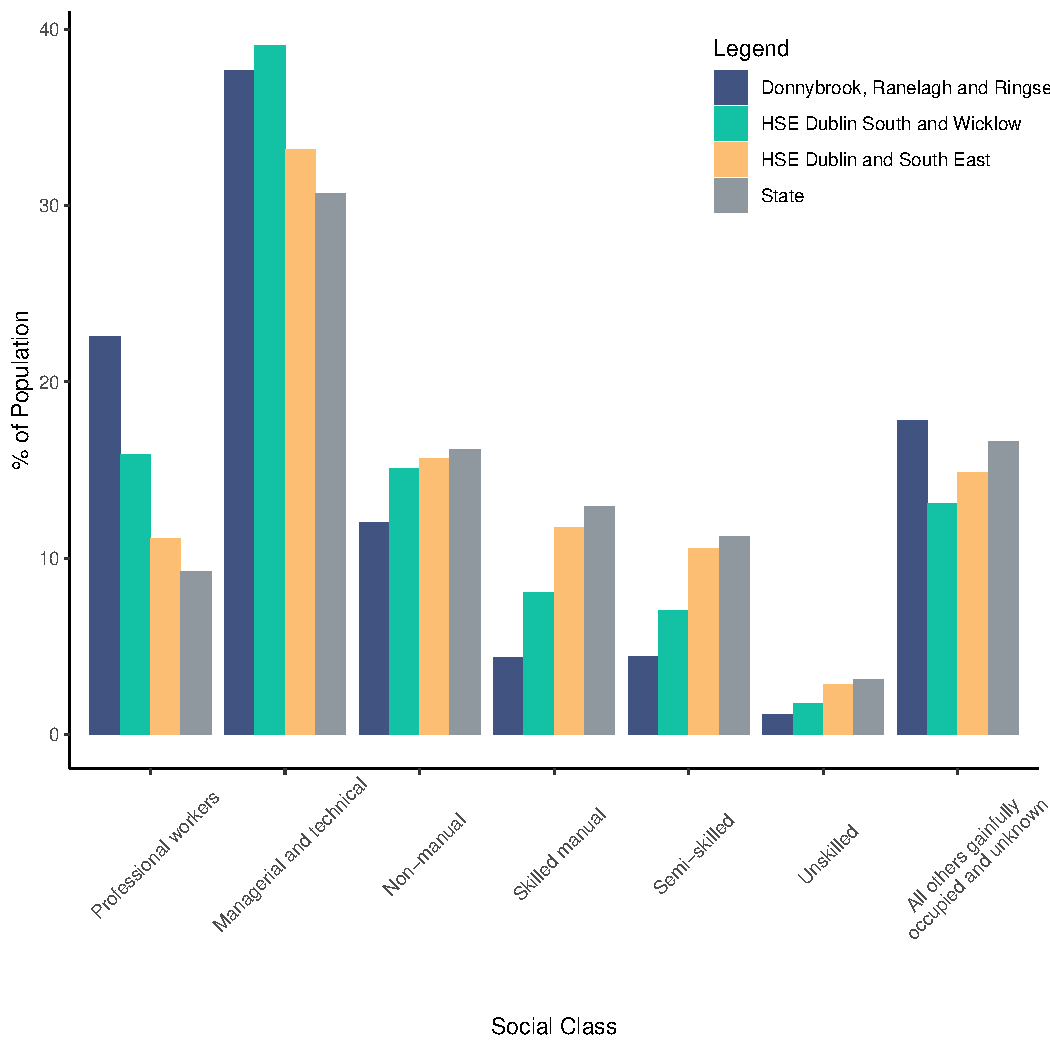
\includegraphics[width = 140mm]{../figures/SocialClassED.pdf}
	\caption{Percentage of Population Aged 15+ by Social Class for West Mayo, IHA, Health Region and State; Census 2022.}
	\label{fig:vbnv}
	\end{figure}

\begin{table}[h]	
\centering
		\begin{tabular}{lTTTTTT}
  \hline
  \textbf{Social Class} & \multicolumn{2}{c}{\textbf{West Mayo}}  & \textbf{IHA} & \textbf{HR} & \textbf{State}\\ 
 \cline{2-3} \\
 & \emph{\textbf{Persons}} & \emph{\textbf{\%}} & \emph{\textbf{\%}} & \emph{\textbf{\%}} & \emph{\textbf{\%}} \\
  \hline
Professional workers & \num{3301} & 8.8 & 7.6& 8.5& 9.3\\
Managerial and technical & \num{11571} & 31.0 & 29.4& 29.7& 30.7\\
Non-manual & \num{5770} & 15.4 & 16.5& 16.0& 16.2\\
Skilled manual & \num{5635} & 15.1 & 15.0& 13.7& 12.9\\
Semi-skilled & \num{4592} & 12.3 & 12.8& 12.3& 11.2\\
Unskilled & \num{1312} & 3.5 & 3.6& 3.3& 3.1\\
All others gainfully occupied and unknown & \num{5187} & 13.9 & 15.0& 16.4& 16.6\\
Total & \num{37368} & 100.0 & 100.0& 100.0& 100.0\\
\hline
       \multicolumn{5}{l}{\href{https://data.cso.ie/table/SAP2022T9T1ED}{https://data.cso.ie/table/SAP2022T9T1ED}} &
\end{tabular}

\caption{Population aged 15+ by Social Class for West Mayo; Census 2022. Percentage breakdowns for IHA, Health Region and State are also provided for comparison purposes.}
\end{table} 
\pagebreak
\begin{itemize}
\item This CHN ranks  14 out of 96 regarding the percentage of the population aged 15+ that are classified as unskilled, while it ranks   2 out of 3 CHNs in its IHA.
\item This CHN ranks  32 out of 96 regarding the percentage of the population aged 15+ that are classified as professional workers, while it ranks   1 out of 3 CHNs in its IHA.
\end{itemize}
\pagebreak
\section{Education}\label{sect:Edu}
\begin{figure}[H]
	\centering
	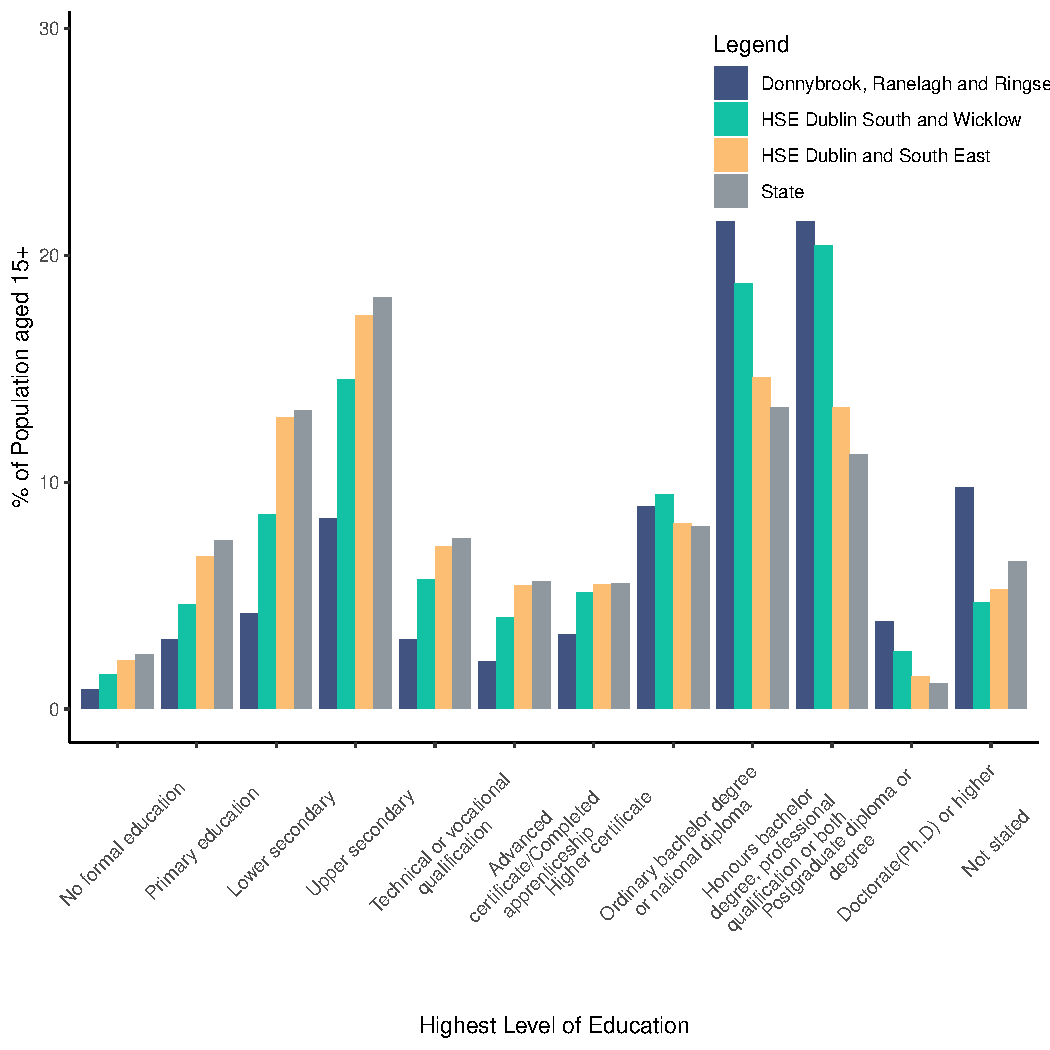
\includegraphics[width = 120mm]{../figures/EduED.pdf}
	\caption{Percentage of Population Aged 15+ by Highest Level of Education Completed for West Mayo; IHA, Health Region and State; Census 2022.}
	\label{fig:vbnv}
	\end{figure}
\begin{table}[h]	
\centering
	\begin{tabular}{lTTTTT}
  \hline
  \textbf{Highest Level of Education Completed} & \multicolumn{2}{c}{\textbf{West Mayo}} & \textbf{IHA}& \textbf{HR} & \textbf{State}\\ 
 \cline{2-3} \\
 & \emph{\textbf{Persons}} & \emph{\textbf{\%}} & \emph{\textbf{\%}} & \emph{\textbf{\%}} \\
  \hline
No formal education & \num{789} &3.1 &3.4&2.9 &2.4 \\
Primary education & \num{2355} &9.1 &9.6 &8.9 &7.4 \\
Lower secondary & \num{3317} &12.9 &14.1&13.6 &13.2 \\
Upper secondary & \num{4986} &19.4 &21.3 &18.7 &18.1 \\
Technical or vocational qualification & \num{1908} &7.4 &7.6&7.6 &7.5 \\
Advanced certificate/Completed apprenticeship & \num{1556} &6.0 &5.9&5.6 &5.6 \\
Higher certificate & \num{1529} &5.9 &5.4&5.6 &5.5 \\
Ordinary bachelor degree or national diploma & \num{2255} &8.8 &8.0&8.2 &8.1 \\
Honours bachelor degree, professional qualification or both & \num{3092} &12.0 &11.3&12.3 &13.3 \\
Postgraduate diploma or degree & \num{2495} &9.7 &8.1&9.9 &11.2 \\
Doctorate(Ph.D) or higher & \num{238} &0.9 &0.6&1.0 &1.1 \\
Not stated & \num{1243} &4.8 &4.8 &5.7 &6.5 \\
Total & \num{25763} &100.0 &100.0 &100.0 &100.0 \\
   \hline
       \multicolumn{5}{l}{\href{https://data.cso.ie/table/SAP2022T10T4ED}{https://data.cso.ie/table/SAP2022T10T4ED}} &
\end{tabular}

\caption{Population aged 15+ by Highest Level of Education Completed for West Mayo; Census 2022. Percentage breakdowns for IHA, Health Region and State are also provided for comparison purposes.}
\end{table} 
\pagebreak
\begin{itemize}
\item This CHN ranks  21 out of 96 regarding the percentage of the population aged 15+ with a highest level of education of Primary or lower, while it ranks  2 out of 3 CHNs in its IHA.
\item This CHN ranks  40 out of 96 regarding the percentage of the population aged 15+ with a highest level of education of Ordinary bachelor degree or national diploma or higher, while it ranks   1 out of 3 CHNs in its IHA.
\end{itemize}
\pagebreak
    
\section{Families}\label{sect:Fam}
\begin{itemize}
\item This CHN ranks  56 out of 96 regarding the percentage of \textbf{family units} with a lone parent (see Detailed Tables section), while it ranks   3 out of 3 CHNs in its IHA.
\end{itemize}
\begin{figure}[H]
	\centering
	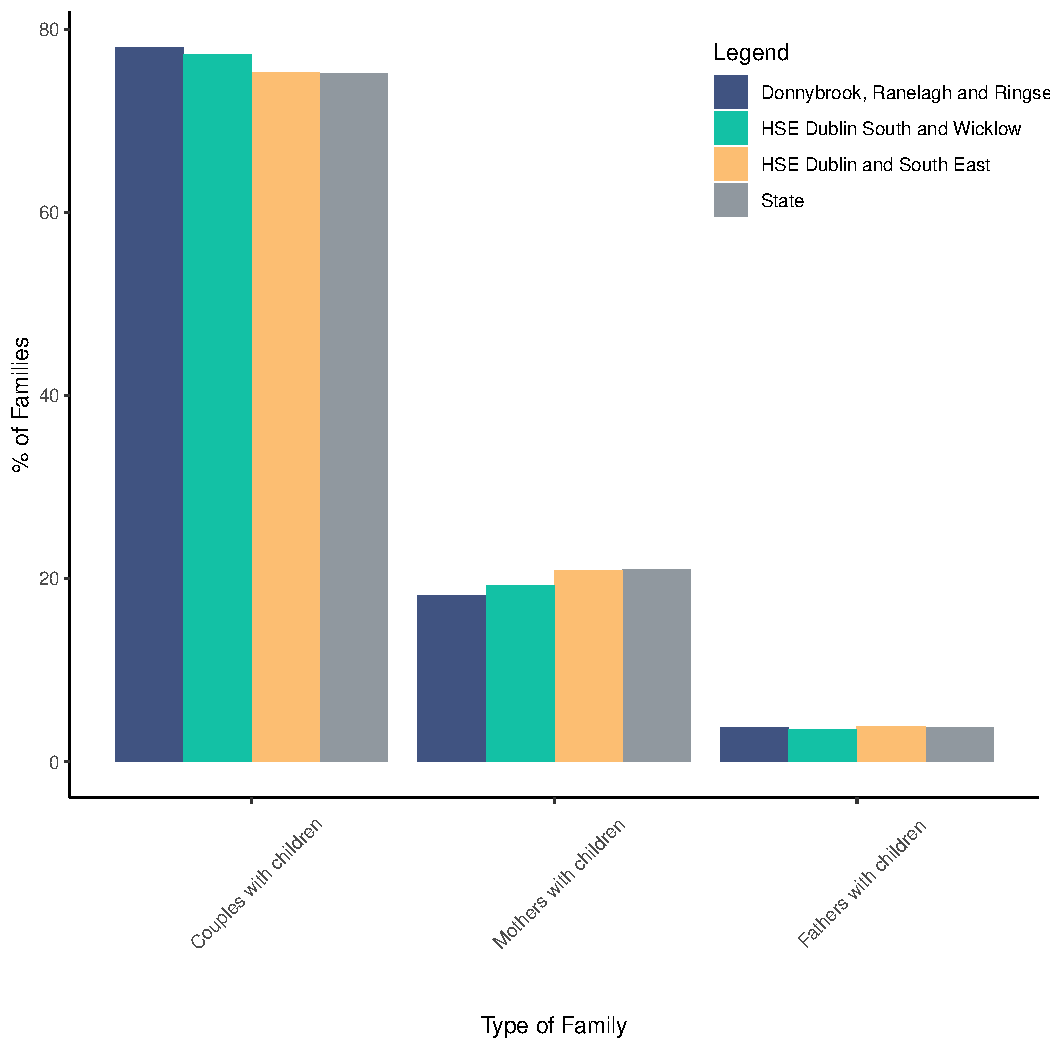
\includegraphics[width = 150mm]{../figures/FamED.pdf}
	\caption{Percentage of Families with Children by Family Type for West Mayo; IHA, Health Region and State; Census 2022.}
	\label{fig:vbnv}
	\end{figure}
	
	
\begin{table}[h]	
\centering
\begin{tabular}{lTTTTT}
  \hline
  \textbf{Type of Family} & \multicolumn{2}{c}{\textbf{West Mayo}} & \textbf{IHA}& \textbf{HR} & \textbf{State}\\ 
 \cline{2-3} \\
 & \emph{\textbf{Families}} & \emph{\textbf{\%}} & \emph{\textbf{\%}} & \emph{\textbf{\%}}& \emph{\textbf{\%}}  \\
  \hline
Couples with Children & \num{4822} &77.9 &76.5 &76.5 &75.2 \\
Mothers with Children & \num{1147} &18.5 &19.5 &19.7 &21.1 \\
Fathers with Children & \num{220} &3.6 &4.0 &3.8 &3.8 \\
All Families & \num{6189} & 100.0 & 100.0  & 100.0 & 100.0 \\
  \hline
       \multicolumn{5}{l}{\href{https://data.cso.ie/table/SAP2022T4T3ED}{https://data.cso.ie/table/SAP2022T4T3ED}}  &
\end{tabular}

\caption{Families with Children by Family Type for West Mayo; 2022. Percentage breakdowns for IHA, Health Region and State are also provided for comparison purposes.}
\end{table} 
\pagebreak

\section{Birthplace}\label{sect:Birth}
\begin{itemize}
\item This CHN ranks  39 out of 96 regarding the percentage of the population that were born outside Ireland, while it ranks  2 out of 3 CHNs in its IHA.
\end{itemize}
\begin{figure}[H]
	\centering
	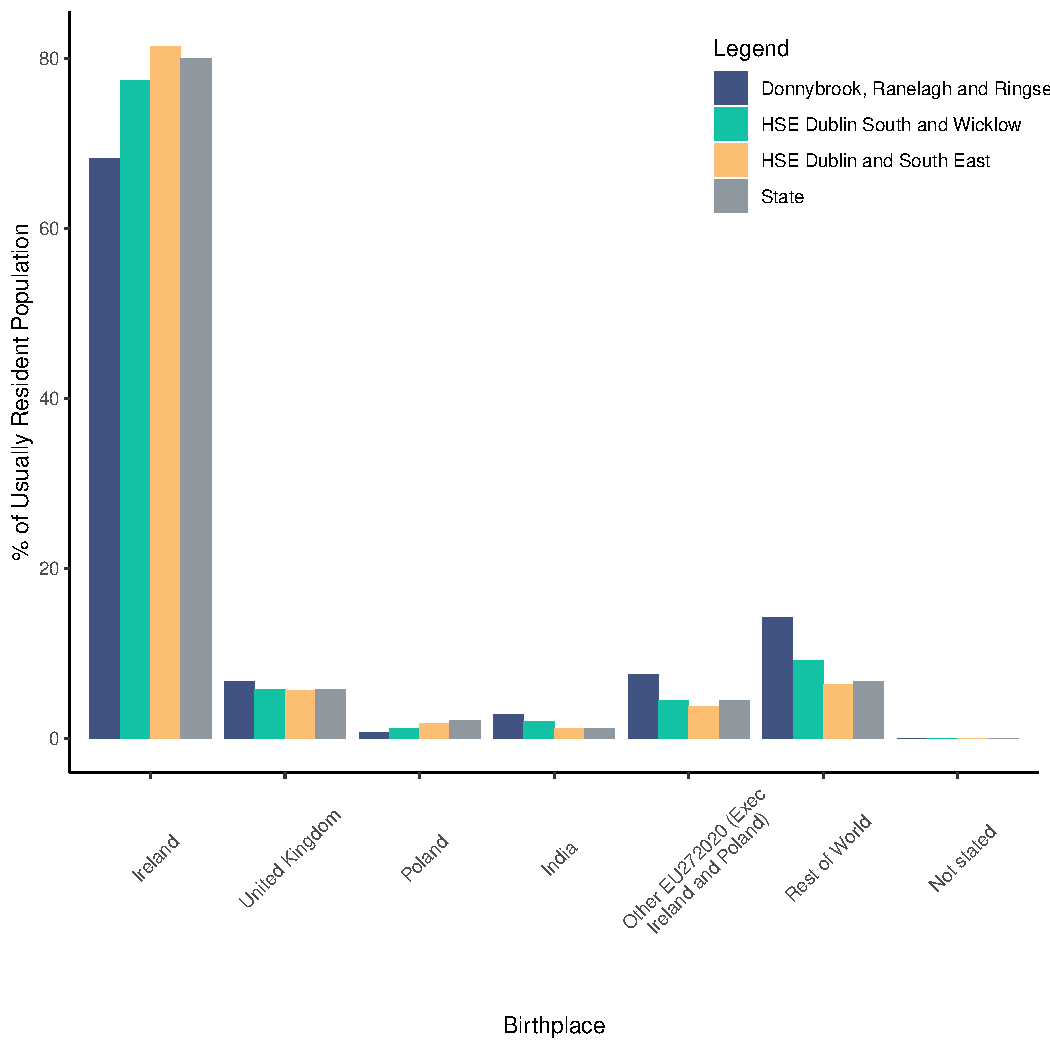
\includegraphics[width = 130mm]{../figures/BirthED.pdf}
	\caption{Percentage of Usually Resident Population by Birthplace for West Mayo; IHA, Health Region and State; Census 2022.}
	\label{fig:vbnv}
	\end{figure}
	
	
\begin{table}[h]	
\centering
	\begin{tabular}{lTTTTT}
  \hline
  \textbf{Birthplace} & \multicolumn{2}{c}{\textbf{West Mayo}} & \textbf{IHA}& \textbf{HR} & \textbf{State}\\ 
 \cline{2-3} \\
 & \emph{\textbf{Persons}} & \emph{\textbf{\%}} & \emph{\textbf{\%}} & \emph{\textbf{\%}}& \emph{\textbf{\%}} \\
  \hline
Ireland & \num{29668} &81.3 &81.4 &80.3 &80.0 \\
United Kingdom & \num{3622} &9.9 &9.4 &9.6 &5.7 \\
Poland & \num{692} &1.9 &1.8 &1.9 &2.1 \\
India & \num{113} &0.3 &0.5 &0.8 &1.1 \\
Other EU272020 (Exec Ireland and Poland) & \num{1093} &3.0&2.9 &2.8 &4.4 \\
Rest of World & \num{1320} &3.6 &4.0 &4.6 &6.7 \\
Not stated & \num{0} &0.0 &0.0 &0.0 &0.0 \\
Total & \num{36508} &100.0 &100.0 &100.0 &100.0 \\
  \hline
       \multicolumn{5}{l}{\href{https://data.cso.ie/table/SAP2022T2T1ED}{https://data.cso.ie/table/SAP2022T2T1ED}} &
\end{tabular}

\caption{Usually Resident Population By Birthplace for West Mayo, Census 2022. Percentage breakdowns for IHA, Health Region and State are also provided for comparison purposes.}
\end{table} 
\pagebreak

\section{Households - Type of Occupancy}\label{sect:Households}
\begin{itemize}
\item This CHN ranks  54 out of 96 regarding the percentage households that are rented from a Local Authority, while it ranks  2 out of the CHNs in its IHA. 
\item This CHNranks  9 out of 96 regarding the percentage of households that are owned outright, while it ranks   2 out of 3 CHNs in its IHA.
\end{itemize}
\begin{figure}[H]
	\centering
	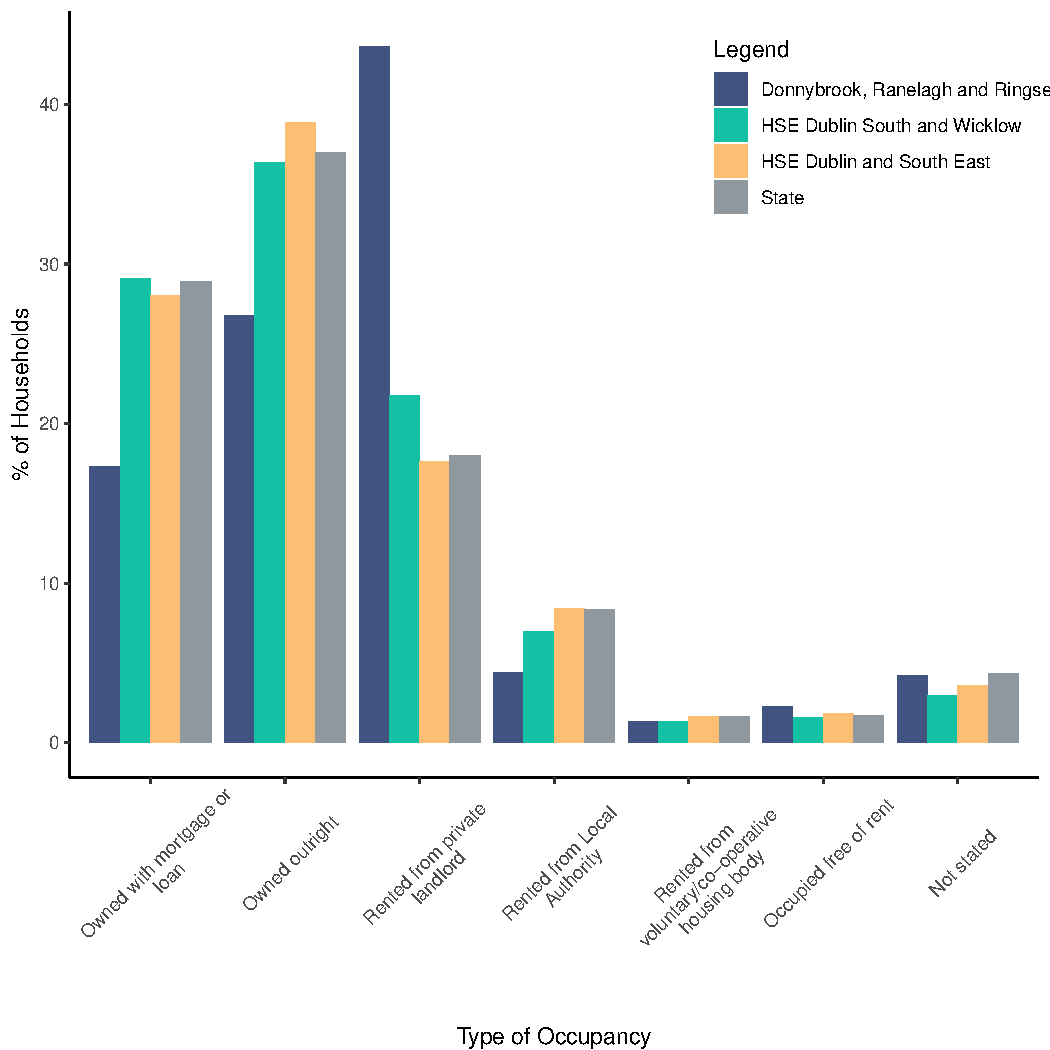
\includegraphics[width = 140mm]{../figures/HouseholdsED.pdf}
	\caption{Percentage of Households by Type of Occupancy for West Mayo, IHA, Health Region and State; Census 2022.}
	\label{fig:vbnv}
	\end{figure}

\begin{table}[h]	
\centering
		\begin{tabular}{lTTTTT}
  \hline
  \textbf{Type of Occupancy} & \multicolumn{2}{c}{\textbf{West Mayo}} & \textbf{HR} & \textbf{State}\\ 
 \cline{2-3} \\
 & \emph{\textbf{Households}} & \emph{\textbf{\%}} & \emph{\textbf{\%}} & \emph{\textbf{\%}} \\
  \hline
Owned with mortgage or loan & \num{3507} & 25.5 & 24.9& 25.7 & 28.9 \\
Owned outright & \num{6602} & 48.0 & 47.9 & 43.6 & 37.0 \\
Rented from private landlord & \num{2026} & 14.7 & 15.2& 16.6 & 18.0 \\
Rented from Local Authority & \num{612} & 4.4 & 4.9 & 6.3 & 8.3 \\
Rented from voluntary/co-operative housing body & \num{102} & 0.7 & 1.0 & 1.1 & 1.6 \\
Occupied free of rent & \num{348} & 2.5 & 2.4 & 2.3 & 1.7 \\
Not stated & \num{568} & 4.1 & 3.7& 4.3 & 4.4 \\
Total & \num{13765} & 100.0 & 100.0& 100.0 & 100.0 \\
\hline
       \multicolumn{5}{l}{\href{https://data.cso.ie/table/SAP2022T6T3ED}{https://data.cso.ie/table/SAP2022T6T3ED}} &
\end{tabular}

\caption{Percentage of Households by Type of Occupancy for West Mayo; Census 2022. Percentage breakdowns for IHA, Health Region and State are also provided for comparison purposes.}
\end{table} 

\pagebreak

\section{Transport}\label{sect:Trans}
\begin{figure}[H]
	\centering
	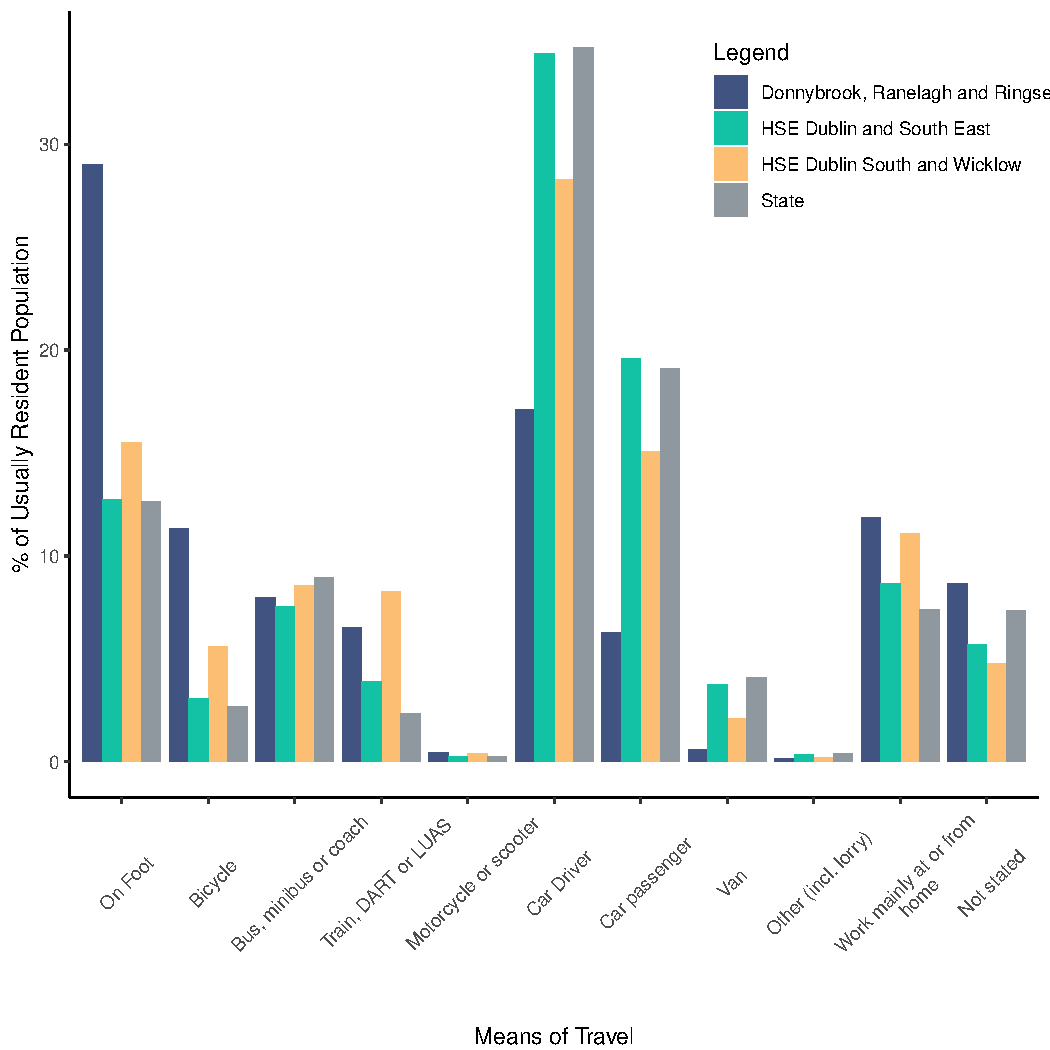
\includegraphics[width = 120mm]{../figures/TravelED.pdf}
	\caption{Percentage of Usually Resident Population by Means of Travel to Work, School, College or Childcare for West Mayo; IHA, Health Region and State; Census 2022.}
	\label{fig:vbnv}
	\end{figure}

\begin{table}[h]	
\centering
		\begin{tabular}{lTTTTTT}
  \hline
  \textbf{Means of travel} & \multicolumn{2}{c}{\textbf{West Mayo}} & \textbf{IHA}& \textbf{HR} & \textbf{State}\\ 
 \cline{2-3} \\
 & \emph{\textbf{Persons}} & \emph{\textbf{\%}} & \emph{\textbf{\%}} & \emph{\textbf{\%}} & \emph{\textbf{\%}} \\
 On Foot & \num{2094} & 8.4 & 8.7& 8.9 & 12.6 \\
Bicycle & \num{258} & 1.0 & 0.9 & 1.3 & 2.7 \\
Bus, minibus or coach & \num{1919} & 7.7 & 7.1 & 8.2 & 9.0 \\
Train, DART or LUAS & \num{65} & 0.3 & 0.3& 0.4 & 2.4 \\
Motorcycle or scooter & \num{20} & 0.1 & 0.1 & 0.1 & 0.3 \\
Car Driver & \num{9960} & 40.1 &  41.0 & 38.5 & 34.7 \\
Car passenger & \num{5528} & 22.3 & 23.5 & 22.9 & 19.1 \\
Van & \num{1713} & 6.9 & 6.6& 5.7 & 4.1 \\
Other (incl. lorry) & \num{155} & 0.6 & 0.6& 0.5 & 0.4 \\
Work mainly at or from home & \num{1798} & 7.2 & 6.0 & 6.9 & 7.4 \\
Not stated & \num{1332} & 5.4 & 5.4 & 6.5 & 7.4 \\
Total & \num{24842} & 100.0 & 100.0& 100.0 & 100.0 \\
  \hline
       \multicolumn{5}{l}{\href{https://data.cso.ie/table/SAP2022T11T1ED}{https://data.cso.ie/table/SAP2022T11T1ED}} &
\end{tabular}

\caption{Percentage of Usually Resident Population by Means of Travel to Work, School, College or Childcare for West Mayo; Census 2022. Percentage breakdowns for IHA, Health Region and State are also provided for comparison purposes.}
\end{table} 

\pagebreak
\begin{itemize}
\item This CHN ranks  60 out of 96 regarding the percentage of the population who travel to work, school, college or childcare on foot or bicycle, while it ranks   2 out of 3 CHNs in its IHA.
\item This CHN ranks  13 out of 96 regarding the percentage of the population who travel to work, school, college or childcare as a car driver, while it ranks   2 out of 3 CHNs in its IHA.
\end{itemize}
\pagebreak
\section{Renewable Energy}\label{sect:RE}
\begin{itemize}
\item This CHN ranks  64 out of 96 regarding the percentage of households with no renewable energy source, while it ranks   3 out of 3 CHNs in its IHA.
\end{itemize}
\begin{figure}[H]
	\centering
	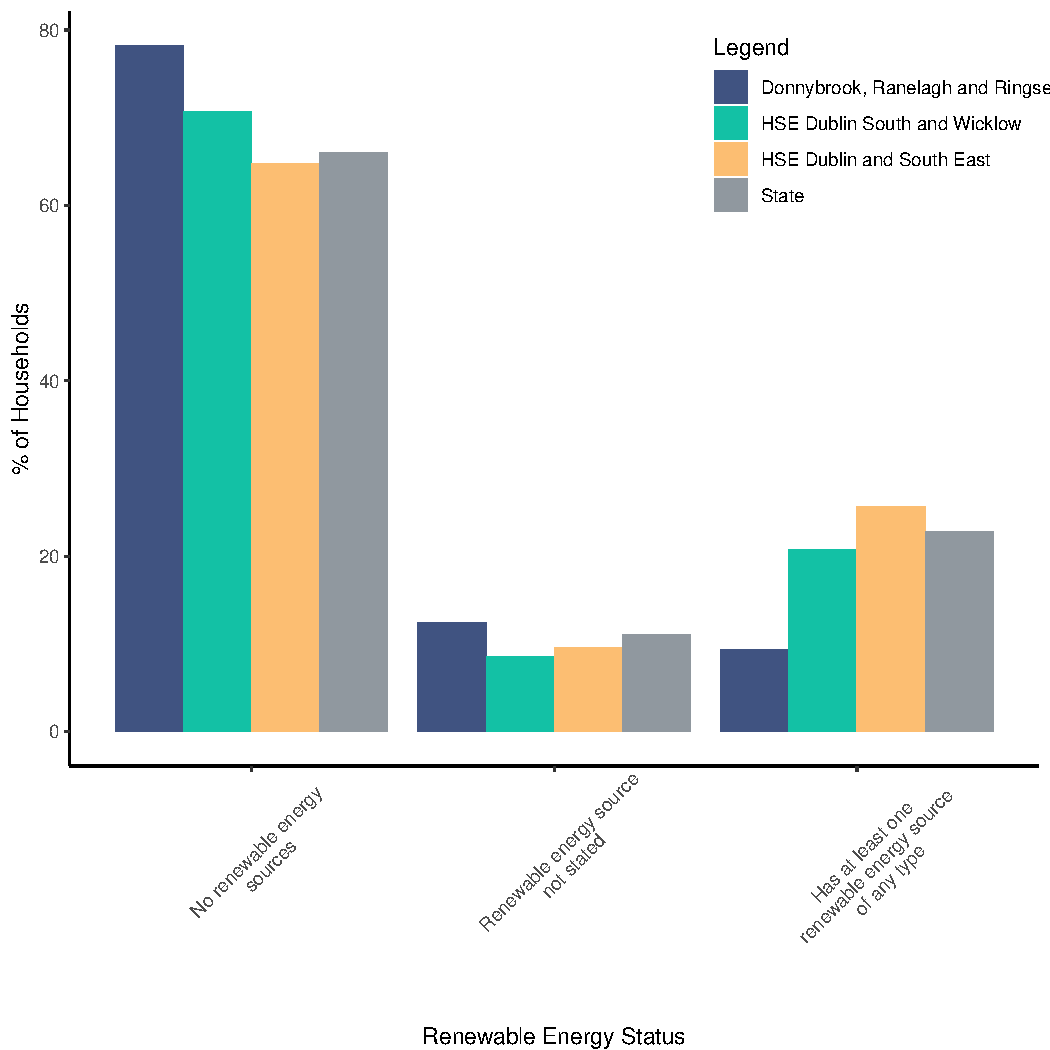
\includegraphics[width = 140mm]{../figures/RenewableEnergyED.pdf}
	\caption{Percentage of Households by Renewable Energy Source for West Mayo; IHA, Health Region and State; Census 2022.}
	\label{fig:vbnv}
	\end{figure}

\begin{table}[h]	
\centering
		\begin{tabular}{lTTTTT}
  \hline
  \textbf{Renewable Energy Source} & \multicolumn{2}{c}{\textbf{West Mayo}} & \textbf{IHA}& \textbf{HR} & \textbf{State}\\ 
 \cline{2-3} \\
 & \emph{\textbf{Households}} & \emph{\textbf{\%}} & \emph{\textbf{\%}} & \emph{\textbf{\%}}& \emph{\textbf{\%}} \\
 All households & \num{13765} & 100.0 & 100.0 & 100.0 & 100.0 \\
  No renewable energy sources & \num{8261} & 60.0 & 64.5& 64.8 & 66.1 \\
   Renewable energy source not stated & \num{1349} & 9.8 & 9.8& 10.7 & 11.0 \\
    Has at least one renewable energy source of any type & \num{4155} & 30.2 & 25.8& 24.5 & 22.9 \\
  \hline
       \multicolumn{5}{l}{\href{https://data.cso.ie/table/SAP2022T6T10ED}{https://data.cso.ie/table/SAP2022T6T10ED}} &
\end{tabular}

\caption{Percentage of Households by Renewable Energy Source for West Mayo; Census 2022. Percentage breakdowns for IHA, Health Region and State are also provided for comparison purposes.}
\end{table} 

\pagebreak

\section{Detailed Tables}\label{sect:ST}
\begin{table}[h]	
\centering
		\begin{tabular}{KTTTT}
  \hline
& \textbf{CHN} & \textbf{IHA} & \textbf{HR} & \textbf{State}\\  
\hline
  \multicolumn{5}{l}{\textbf{Age (Percentage of population (excl. Dependency ratios))} }\\ 
\hline
    \multicolumn{5}{l}{\textbf{Education (Percentage of those aged 15+)}}\\
    \arrayrulecolor{black}\hline
No formal education & 3.1& 3.4& 2.9& 2.4\\
Primary education & 9.1& 9.6& 8.9& 7.4\\
Lower secondary & 12.9& 14.1& 13.6& 13.2\\
Upper secondary & 19.4& 21.3& 18.7& 18.1\\
Technical or vocational qualification  & 7.4& 7.6& 7.6& 7.5\\
Advanced certificate/Completed apprenticeship & 6.0& 5.9& 5.6& 5.6\\
Higher certificate & 5.9& 5.4& 5.6& 5.5\\
Ordinary bachelor degree or national diploma & 8.8& 8.0& 8.2& 8.1\\
Hns bach. degree, prof. qual. or both & 12.0& 11.3& 12.3& 13.3\\
Postgraduate diploma or degree &  9.7&  8.1&  9.9& 11.2\\
Doctorate(Ph.D) or higher & 0.9& 0.6& 1.0& 1.1\\
  \arrayrulecolor{black}\hline
    \multicolumn{5}{l}{\textbf{Employment (Percentage of those aged 15+)}}\\ 
    \arrayrulecolor{black}\hline
At work & 53.7& 52.3& 53.6& 56.1\\
Looking for first regular job & 0.5& 0.8& 0.8& 0.8\\
short Term Unemployed  & 1.5& 1.6& 1.7& 1.7\\
Long Term Unemployed  & 2.2& 2.7& 2.7& 2.6\\
Student  &  9.6&  9.7& 11.1& 11.1\\
Looking after home/family   & 6.6& 6.7& 6.4& 6.6\\
Retired  & 21.2& 20.7& 18.4& 15.9\\
Unable to work - perm. sickness or disability & 4.0& 4.8& 4.8& 4.6\\
\hline
    \multicolumn{5}{l}{\textbf{Employment (Percentage of those at work)}}\\
    \hline
Agriculture, forestry and fishing  & 6.6& 6.2& 5.3& 3.5\\
Building and construction & 6.7& 6.7& 6.1& 5.8\\
Manufacturing industries & 16.2& 15.7& 14.1& 11.8\\
Commerce and trade  & 19.6& 20.4& 19.8& 23.8\\
Transport and communications  & 5.0& 4.9& 6.4& 9.2\\
Public administration & 5.6& 6.5& 6.5& 5.7\\
Professional services & 21.6& 24.2& 26.1& 24.5\\
%Other & & 15.7& 15.8\\
\arrayrulecolor{black}\hline
    \multicolumn{5}{l}{\textbf{Social Class (Percentage of population)}}\\ 
    \arrayrulecolor{black}\hline
Professional workers  & 8.8& 7.6 & 8.5& 9.3\\
Managerial and technical & 31.0& 29.4& 29.7& 30.7\\
Non-manual & 15.4& 16.5& 16.0& 16.2\\
Skilled manual & 15.1& 15.0& 13.7& 12.9\\
Semi-skilled & 12.3& 12.8& 12.3& 11.2\\
Unskilled  & 3.5& 3.6& 3.3& 3.1\\
\end{tabular}
\end{table}
\pagebreak
\begin{table}[h]	
\centering
		\begin{tabular}{KTTTT}
  \arrayrulecolor{black}\hline
& \textbf{CHN} & \textbf{IHA} & \textbf{HR}& \textbf{State}\\ 
\hline
   \multicolumn{5}{l}{\textbf{Families (Percentage of family units)}}\\ 
   \arrayrulecolor{black}\hline
Families without children & 34.4& 33.4&32.1& 30.8\\
Families with 1 child & 25.3& 26.3&26.2& 27.1\\
Families with 2 children & 22.4& 22.6&23.8& 25.3\\
Families with 3 children & 13.0& 12.3&12.7& 12.3\\
Families with 4 children & 3.8& 4.1& 4.0& 3.5\\
Families with 5 or more children & 1.1& 1.3&1.3& 1.0\\
    \arrayrulecolor{lightgray}\hline
Couples with children & 51.1& 51.0&52.0& 52.0\\
Lone parent (mother) & 12.2& 13.0& 13.4& 14.6\\
Lone parent (father) & 2.3& 2.6& 2.6& 2.6\\
    \arrayrulecolor{lightgray}\hline
Pre-family families & 7.1& 6.8&7.6& 9.3\\
Empty nest families & 11.5& 11.2& 10.7&  9.4\\
Retired families & 15.8& 15.4&13.8& 12.0\\
Per-school families & 7.2& 7.5& 7.8& 8.1\\
Early school families & 9.1& 9.2&9.6& 9.9\\
Pre-adolescent families & 11.1& 10.9&11.5& 11.9\\
Adolescent families & 12.2& 12.1&12.6& 12.3\\
Adult families & 51.1& 26.9& 26.4& 27.0\\
    \arrayrulecolor{lightgray}\hline
Families with youngest child aged 0 - 4 & 22.6& 23.4&24.0& 14.6\\
Families with youngest child aged 5 - 9 & 17.8& 17.5&17.9& 18.1\\
Families with youngest child aged 10 - 14 & 16.5& 16.1&16.7& 16.9\\
Families with youngest child aged 15 - 19 & 14.4& 14.0&13.8& 13.6\\
Families with youngest child aged 20 and over & 28.7& 29.1&27.7& 27.5\\
\arrayrulecolor{black}\hline
    \multicolumn{5}{l}{\textbf{Health (Percentage of population)}}\\ 
    \arrayrulecolor{black}\hline
Very good general health & 52.2& 51.4&52.3& 53.2\\
Good general health & 32.0& 32.1& 30.8& 29.7\\
Fair general health &  9.5& 10.2& 9.6&  8.6\\
Bad general health & 1.4& 1.6&1.5& 1.4\\
Very bad general health & 0.3& 0.3&0.3& 0.3\\
    \arrayrulecolor{lightgray}\hline
Persons who smoke & 12.1& 12.4&12.5& 13.1\\
    \arrayrulecolor{lightgray}\hline
With a disability (to some or to a great extent) & 21.5& 21.8&21.8& 21.5\\
\arrayrulecolor{black}\hline
    \multicolumn{5}{l}{\textbf{Household composition (Percentage of Private Households)}}\\ 
    \arrayrulecolor{black}\hline
Married couple households & 18.0& 17.7& 16.4& 14.9\\
Cohabiting couple households & 4.1& 3.6& 3.7& 4.3\\
Married couple with children households & 29.4& 28.9& 29.6& 29.4\\
Cohabiting couple with children households & 3.5& 3.7& 3.8& 4.3\\
One parent family (father) with  children households & 1.3& 1.5& 1.5& 1.5\\
One parent family (mother) and children households & 7.0& 7.6& 7.8& 8.5\\
Couple and others households  & 0.9& 0.8& 1.1& 1.5\\
Two or more non-related persons households & 3.2& 2.8& 4.5& 5.4\\
    \arrayrulecolor{lightgray}\hline
1 person households & 26.8& 27.9& 26.1& 23.1\\
2 person households & 30.4& 29.9& 29.0& 29.0\\
3 person households & 15.5& 15.6& 16.6& 17.9\\
4 person households & 14.4& 14.0& 15.3& 16.9\\
5 person households & 8.8& 8.3& 8.7& 8.9\\
6 person households & 3.0& 3.1& 3.1& 3.0\\
7 person households & 0.7& 0.9& 0.8& 0.8\\
8 or more person households & 0.3& 0.3& 0.4& 0.4\\
\arrayrulecolor{black}\hline
    \multicolumn{5}{l}{\textbf{Housing (Percentage of permanent dwellings)}}\\ 
    \arrayrulecolor{black}\hline
Occupied & 71.4& 76.8& 78.9& 87.4\\
Temporarily absent & 1.2& 1.4& 1.6& 1.6\\
Unoccupied holiday homes & 16.3&  8.8&  8.0&  3.2\\
Other vacant dwellings & 11.1& 13.1& 11.6&  7.7\\
\hline
\end{tabular}
\end{table}
\pagebreak
\begin{table}[h]	
\centering
		\begin{tabular}{KTTTT}
 \arrayrulecolor{black} \hline
& \textbf{CHN} & \textbf{IHA}& \textbf{HR} & \textbf{State}\\ 
\hline
    \multicolumn{5}{l}{\textbf{Housing (Percentage of permanent private households)}}\\ 
    \arrayrulecolor{black}   \hline
Owned with mortgage or loan & 25.5& 24.9& 25.7& 28.9\\
Owned outright & 48.0& 47.9& 43.6& 37.0\\
Rented from private landlord & 14.7& 15.2& 16.6& 18.0\\
Rented from Local Authority & 4.4& 4.9& 6.3& 8.3\\
Rented from voluntary/co-operative housing body & 0.7& 1.0& 1.1& 1.6\\
Occupied free of rent & 2.5& 2.4& 2.3& 1.7\\
    \arrayrulecolor{lightgray}\hline
1 room & 0.3& 0.3& 0.2& 0.5\\
2 rooms & 2.5& 2.3& 2.5& 3.9\\
3 rooms & 6.4& 5.8& 6.3& 8.0\\
4 rooms &  9.3&  9.3&  9.4& 11.0\\
5 rooms & 20.1& 22.0& 21.4& 23.8\\
6 rooms & 22.7& 23.3& 22.2& 19.9\\
7 rooms & 17.0& 16.5& 16.2& 14.0\\
8 or more rooms & 19.4& 18.3& 19.0& 15.8\\
    \arrayrulecolor{lightgray}\hline
No central heating & 1.3& 1.1& 1.1& 1.2\\
    \arrayrulecolor{lightgray}\hline
Public main water supply & 55.2& 60.7& 70.9& 80.1\\
Group scheme with public source water supply & 16.5& 15.1& 10.4&  4.3\\
Group scheme with private source water supply & 19.1& 16.9&  9.3&  3.4\\
Other private source water supply & 7.3& 5.6& 7.2& 9.9\\
No water supply & 0.2& 0.1& 0.2& 0.1\\
\arrayrulecolor{black}\hline
    \multicolumn{4}{l}{\textbf{Housing (Percentage of private households)}}\\ 
    \arrayrulecolor{black}\hline
House/Bungalow & 93.5& 94.7& 92.5& 86.7\\
Flat/Apartment &  6.2&  5.0&  7.2& 13.0\\
Bed-Sit & 0.0& 0.0& 0.1& 0.1\\
Caravan/Mobile home & 0.2& 0.2& 0.3& 0.2\\
    \arrayrulecolor{lightgray}\hline
Built Pre 1919 & 8.1& 6.5& 6.9& 8.4\\
Built 1919 - 1945 & 7.8& 8.1& 5.9& 6.2\\
Built  1946 - 1960 & 6.0& 6.8& 5.8& 7.2\\
Built  1961 - 1970 & 4.2& 4.8& 5.0& 6.7\\
Built  1971 - 1980 & 10.6& 11.7& 11.3& 12.2\\
Built  1981 - 1990 & 10.9& 12.0& 11.5& 10.1\\
Built  1991 - 2000 & 15.8& 15.7& 16.0& 14.5\\
Built  2001 - 2010 & 27.0& 25.9& 29.0& 24.5\\
Built  2011 - 2015 & 3.2& 2.9& 2.9& 2.7\\
Built  2016 or later & 4.2& 3.5& 3.4& 5.1\\
\arrayrulecolor{black}\hline
    \multicolumn{5}{l}{\textbf{Marital Status (Percentage of population)}}\\
    \arrayrulecolor{black}\hline
Single & 49.3& 50.2& 52.1& 53.9\\
Married (incl. same sex civil partnership) & 40.7& 39.7& 38.6& 37.1\\
Separated  & 2.3& 2.4& 2.3& 2.3\\
Divorced  & 2.7& 2.6& 2.5& 2.6\\
Widowed & 5.0& 5.1& 4.5& 4.1\\
\arrayrulecolor{black}\hline
    \multicolumn{4}{l}{\textbf{Migration and ethnicity (Percentage of population)}}\\ 
   \arrayrulecolor{black} \hline
Speak english not well & 1.0& 1.3& 1.2& 1.6\\
Speak english not at all & 0.1& 0.3& 0.2& 0.3\\
\arrayrulecolor{black}\hline
    \multicolumn{4}{l}{\textbf{Occupation (Percentage of those at work or unemployed)}}\\
   \arrayrulecolor{black} \hline
Managers, directors and senior officials & 8.0& 7.0& 6.8& 7.7\\
Professional occupations & 18.3& 17.6& 19.8& 20.3\\
Associate professional and technical occupations & 10.6&  9.7& 10.2& 11.7\\
Administrative and secretarial occupations & 8.1& 8.8& 9.0& 9.2\\
Skilled trades occupations & 17.9& 16.9& 15.0& 12.6\\
Caring, leisure and other service occupations & 7.3& 8.2& 8.1& 7.4\\
Sales and customer service occupations & 5.6& 6.4& 5.9& 6.2\\
Process, plant and machine operatives & 8.1& 9.1& 8.4& 6.9\\
Elementary occupations & 9.1& 8.7& 8.0& 8.2\\
\arrayrulecolor{black}\hline
\end{tabular}
\end{table}
\pagebreak
\begin{table}[h]	
\centering
		\begin{tabular}{KTTTT}
 \arrayrulecolor{black} \hline
& \textbf{CHN} & \textbf{IHA} & \textbf{HR}& \textbf{State}\\ 
 \arrayrulecolor{black} \hline
    \multicolumn{5}{l}{\textbf{Migration and ethnicity (Percentage of usually resident population)}}\\ 
    \arrayrulecolor{black}\hline
Ireland - Birthplace & 81.3& 81.4& 80.3& 80.0\\
UK - Birthplace & 9.9& 9.4& 9.6& 5.7\\
Poland - Birthplace & 1.9& 1.8& 1.9& 2.1\\
India - Birthplace & 0.3& 0.5& 0.8& 1.1\\
Other EU28 - Birthplace & 3.0& 2.9& 2.8& 4.4\\
Rest of world - Birthplace & 3.6& 4.0& 4.6& 6.7\\
    \arrayrulecolor{lightgray}\hline
White Irish & 83.9& 82.8& 81.3& 76.6\\
White Irish Traveller & 0.4& 1.0& 1.0& 0.6\\
Other White & 9.3& 8.8& 8.3& 9.9\\
Black or Black Irish & 0.2& 0.6& 0.9& 1.5\\
Asian or Asian Irish & 1.1& 1.7& 2.1& 3.3\\
Other ethnic or cultural background & 1.0& 1.4& 1.5& 2.0\\
    \arrayrulecolor{lightgray}\hline
Usual residence 1 year before census day - Outside Ireland & 1.5& 1.3& 1.5& 1.8\\

\arrayrulecolor{black}\hline
    \multicolumn{5}{l}{\textbf{Socio-economic group of ref. person (percentage of private households)}}\\ 
    \arrayrulecolor{black}\hline
A Employers and managers & 11.2& 10.2& 10.5& 12.9\\
B Higher professional & 1.6& 1.2& 1.3& 1.5\\
C Lower professional & 5.0& 4.6& 5.6& 6.3\\
D Non-manual & 31.0& 31.4& 32.9& 34.2\\
E Manual skilled & 8.7& 9.6& 8.5& 8.5\\
F Semi-skilled & 8.4& 9.1& 8.4& 7.7\\
G Unskilled & 3.7& 3.9& 3.5& 3.2\\
H Own account workers & 5.6& 4.7& 4.5& 4.0\\
I Farmers & 6.6& 6.0& 5.0& 3.1\\
J Agricultural workers & 2.4& 2.3& 2.0& 1.2\\
Z All others gainfully occupied and unknown & 15.9& 17.1& 18.0& 17.5\\
\hline
\arrayrulecolor{black}\hline
    \multicolumn{5}{l}{\textbf{Transport (Percentage of population agCHN 5+)}}\\ 
   \arrayrulecolor{black} \hline
No motor car (percentage of households) &  8.6& 10.6& 10.8& 
13.4\\
    \arrayrulecolor{lightgray}\hline 
\emph{Travel to work, school, College or childcare:} & & & \\
\quad On Foot &  8.4&  8.7&  8.9& 12.6\\ 
\quad By Bicycle & 1.0& 0.9& 1.3& 2.7\\ 
\quad By Bus, minibus or coach & 7.7& 7.1& 8.2& 9.0\\
\quad By Train, DART or LUAS & 0.3& 0.3& 0.4& 2.4\\
\quad By Motorcycle or scooter & 0.1& 0.1& 0.1& 0.3\\
\quad Car driver & 40.1 & 41.0& 38.5& 34.7\\
\quad Car passenger & 22.3& 23.5& 22.9& 19.1\\
\quad By Van & 6.9& 6.6& 5.7& 4.1\\
\quad By Other (incl. lorry) & 0.6& 0.6& 0.5& 0.4\\
    \arrayrulecolor{lightgray}\hline
Work mainly at or from home & 7.2& 6.0& 6.9& 7.4\\
Journey time to work, school or college is Under 15 mins & 38.9& 40.3& 35.9& 29.4\\
Journey time to work, school or college is 1/4 hour - under 1/2 hour & 25.1& 26.4& 27.6& 28.1\\
Journey time to work, school or college is 1/2 hour - under 3/4 hour & 14.9& 13.4& 15.4& 17.3\\
Journey time to work, school or college is 3/4 hour - under 1 hour & 5.4& 4.3& 4.7& 5.9\\
Journey time to work, school or college is 1 hour - under 1 1/2 hours & 5.0& 4.8& 4.3& 6.1\\
Journey time to work, school or college is 1 1/2 hours and over & 2.1& 2.3& 2.2& 2.5\\
\arrayrulecolor{black}\hline
    \multicolumn{5}{l}{\textbf{Other}}\\ 
    \arrayrulecolor{black}\hline
Has renewable energy source (percentage of permanent private households) & 30.2& 25.8& 24.5& 22.9\\
    \arrayrulecolor{lightgray}\hline
Volunteers (percentage of population) & 18.5& 16.9& 15.6& 13.8\\
    \arrayrulecolor{lightgray}\hline
No internet connection& 12.7& 13.4& 11.7&  8.7\\
\arrayrulecolor{black}\hline
\end{tabular}
\end{table}


\end{document}
